\documentclass[journal]{IEEEtran}

\usepackage[T1]{fontenc}
\usepackage{lmodern}
\usepackage[utf8]{inputenc}
\IfFileExists{cite.sty}{\usepackage{cite}}{}
\usepackage{amsmath}
\usepackage{array}
\IfFileExists{booktabs.sty}{%
  \usepackage{booktabs}%
}{%
  \newcommand{\toprule}{\hline}
  \newcommand{\midrule}{\hline}
  \newcommand{\bottomrule}{\hline}
}
\usepackage{tabularx}
\usepackage{url}
\usepackage{xcolor}
\IfFileExists{microtype.sty}{\usepackage{microtype}}{}
\usepackage{graphicx}
\usepackage{tikz}
\usetikzlibrary{arrows.meta,positioning,fit,backgrounds}
\IfFileExists{pgfplots.sty}{\usepackage{pgfplots}\pgfplotsset{compat=1.16}}{}
\graphicspath{{figures/}}

\newcolumntype{Y}{>{\raggedright\arraybackslash}X}
\newcommand{\artifact}[1]{\texttt{#1}}
\newcommand{\thingid}{\artifact{building:floor1:elevator}}
\newcommand{\mqttid}{\artifact{building-floor1-elevator}}
\newcommand{\topicbase}{\artifact{elevator/\{id\}/}}

\begin{document}

\title{Safety-Gated Agentic Digital Twin Architecture for Smart Elevator Monitoring and Control}

\author{Zaouidi~Abderrahmane,
        Bengherbia~Mohamed~Hachem,
        and~Mounir~Bouhedda%
% TODO(human): confirm the official lab name. ``LSEA'' matches the French
% ``Laboratoire des Syst\`emes \'Electroniques Avanc\'es''; the English
% expansion below is provided for convenience.
\thanks{The authors are with the Laboratory of Advanced Electronic Systems (LSEA), University of M\'ed\'ea, M\'ed\'ea, Algeria.}%
\thanks{Corresponding authors: Zaouidi Abderrahmane, Bengherbia Mohamed Hachem, and Bouhedda Mounir. E-mails: abdelrahmenzaouidi@gmail.com, Mohamed.bengherbia26@gmail.com, bouhedda.mounir@univ-medea.dz.}}

\markboth{Draft journal article prepared from the master's thesis, June 2026}%
{Zaouidi \MakeLowercase{\textit{et al.}}: Safety-Gated Agentic Digital Twin Architecture}

\maketitle

\begin{abstract}
Connected elevator supervision requires more than telemetry dashboards: the operational state, command authority, security posture, and maintenance logic must be separated and auditable. This paper presents a laboratory-scale smart elevator digital-twin platform built around a four-floor, single-cabin ESP32-S3 prototype and a self-hosted Industrial-IoT stack. The architecture uses Eclipse Mosquitto for authenticated MQTT transport, a Node.js bridge for MQTT-to-Eclipse-Ditto synchronization, Eclipse Ditto as the operational source of truth, PostgreSQL/TimescaleDB for historical and audit records, n8n workflows for bounded agentic automation, an adaptive dispatch policy engine, and a Next.js SCADA dashboard. The central contribution is a safety-gated command path in which every operator or agent action is first represented as Ditto command intent, evaluated by a deterministic rule-based gate, persisted for audit, forwarded by the bridge, and still constrained by firmware-side interlocks. The ``agentic AI'' layer is therefore bounded: workflows analyze, route, explain, and audit, while safety-critical admission and dispatch authority remain deterministic; the optional local language model is explanatory only, and the machine-learning dispatch challenger runs in shadow mode. Validation evidence from the repository and thesis package shows 127 passing automated software assertions, MQTT authentication and ACL enforcement, live Ditto/database exports, nine live command-decision rows with zero Ditto writes for rejected commands, and documented prototype integration. Instrumented end-to-end latency and ESP32 resource profiling are identified as future work.
\end{abstract}

\begin{IEEEkeywords}
Digital twin, smart elevator, Industrial Internet of Things, Eclipse Ditto, MQTT, SCADA, agentic AI, safety gate.
\end{IEEEkeywords}

\section{Introduction}

Elevators are safety-oriented cyber-physical systems whose availability affects mobility, emergency access, maintenance cost, and building security. Connected supervision can provide earlier visibility into overload, vibration, overheating, door faults, unauthorized access, and degraded components. However, connectivity also increases the attack surface: brokers, workflow engines, dashboards, digital-twin APIs, and configuration endpoints become part of the operational safety boundary.

Many laboratory IoT systems present telemetry directly to a dashboard or allow a web application to publish device commands. That pattern is inappropriate for a safety-oriented elevator platform. In this work, the dashboard never controls the device directly. MQTT transports device telemetry and device-facing commands, but Eclipse Ditto is the operational source of truth. Commands from operators or agents become Ditto intent only after deterministic safety validation, database logging, and audit recording. The bridge then forwards accepted intent to the device over authenticated MQTT, and the firmware or simulator applies local interlocks before actuation.

The article is framed as an architecture and systems paper, not as an optimization benchmark. The prototype is a rigorous laboratory platform, not a certified industrial elevator controller. We adopt the evidence boundary of the thesis validation package: software artifacts and live-stack traces are reported as validated, while physical mechanisms without captured serial, video, or log measurements are reported as documented integration or future work.

The main contributions are:
\begin{itemize}
  \item a reproducible self-hosted Industrial-IoT architecture for a smart elevator digital twin using ESP32-S3, Mosquitto, Eclipse Ditto, PostgreSQL/TimescaleDB, n8n, a Node.js bridge, and a Next.js SCADA dashboard;
  \item a command-authority discipline in which Ditto is the state authority, MQTT is the transport layer, and every command follows a deterministic safety-gated intent path;
  \item a bounded agentic automation layer composed of surveillance, analysis, control, security/maintenance, notification, optimization, and audit workflows, with no generative-AI authority over safety-critical commands;
  \item an adaptive dispatch policy engine where deterministic Brain A is active and the machine-learning Brain B remains a shadow challenger pending future evidence and human approval;
  \item an evidence-driven validation summary that separates software PASS results, documented hardware integration, and prototype timing from the instrumented measurements deferred to future work.
\end{itemize}

The rest of the paper is organized as follows. Section II reviews related work and the research gap. Section III presents the system architecture and command path. Section IV describes the implementation. Section V reports validation evidence and the measurements deferred to future work. Sections VI and VII discuss scope, limitations, and future hardening, and Section VIII concludes.

\section{Related Work and Research Gap}

\subsection{Digital Twins for Cyber-Physical Systems}

Digital twins provide persistent virtual representations of physical assets synchronized with operational data and context. The concept has evolved from early virtual-counterpart and aerospace paradigms into industrial reference architectures and surveys of enabling technologies \cite{grieves2017digitalTwin,glaessgen2012digitalTwin,tao2019digitalTwin,qi2021enablingDT}. Kritzinger et al. distinguish digital models, digital shadows, and digital twins according to the degree of automated bidirectional data flow \cite{kritzinger2018digitalTwin}. IoT-oriented reviews identify recurring limitations: heterogeneous models, fragmented tooling, weak reproducibility, and insufficient integration of security and control feedback paths \cite{minerva2020digitalTwinIot,fuller2020digitalTwin}.

Eclipse Ditto is useful in this context because it models each asset as a Thing with attributes, features, and policies, consistent with web-of-things concepts for addressable properties and actions \cite{eclipseDittoDocs,w3cWoTArchitecture2023}. This supports an explicit separation between slowly varying metadata and subsystem state. In the present platform, Ditto is not a dashboard cache. It is the operational state authority through which dashboards, agents, dispatch logic, and command intent are coordinated.

\subsection{Elevator IoT and Predictive Maintenance}

Elevator monitoring commonly emphasizes condition indicators such as door cycles, vibration, load, temperature, power, availability, and incident frequency. Predictive-maintenance surveys show the shift from scheduled maintenance to condition-based and predictive strategies, often using digital twins or machine-learning models \cite{vanDinter2022predictiveMaintenance,zonta2020predictiveMaintenance}. These approaches are valuable, but laboratory prototypes rarely have long-duration labeled failure data. The present work therefore implements predictive maintenance as deterministic decision support: risk flags, work-order state, and recommended actions are generated from auditable rules rather than from an unvalidated failure-probability model.

\subsection{Messaging, Security, and Multi-Agent Automation}

MQTT is a lightweight publish/subscribe protocol suitable for constrained devices and asynchronous IoT systems \cite{hunkeler2008mqtt,oasisMqtt2019,naik2017messaging}. Mosquitto provides a practical open-source broker implementation \cite{light2017mosquitto}. The protocol alone does not provide a complete industrial security posture, so authenticated identities, topic ACLs, TLS, credential lifecycle management, monitoring, and segmentation are required in safety-relevant deployments \cite{nistSp80082,iec62443SecurityLevels2013,nistCsf2024,hassija2019iotSecurity}.

Multi-agent systems distribute responsibility among cooperating entities \cite{wooldridge2009multiAgent,dorri2018multiAgent}. Recent language-model agent literature expands this vocabulary, but a safety-oriented elevator platform cannot allow opaque model outputs to authorize physical commands \cite{xi2023llmAgents,wang2024llmAgents}. We therefore adopt \emph{bounded autonomy} as the primary framing and define ``agentic'' narrowly, once, for use thereafter: workflow-based automation with explicit roles and deterministic authority boundaries. Under this definition the optional local language model produces human-readable explanation only and is not part of the command-admission predicate.

\subsection{Runtime Assurance and Safety Monitors}

The closest prior art to this paper's contribution is not digital-twin modeling but runtime assurance and safety monitoring for cyber-physical and autonomous systems. The Simplex architecture established the pattern of a small, high-assurance decision module that constrains a complex, less-trusted controller so the system stays within a safety envelope \cite{sha2001simplex}. Runtime verification monitors an executing system against formally specified properties and reacts when they are violated \cite{leucker2009runtimeVerification}. For learning-enabled control, shielding synthesizes a reactive safety layer that filters or corrects actions before they reach the plant, so an unverified policy can never drive the system into an unsafe state \cite{alshiekh2018shielding}. These mechanisms share a lineage with supervisory control of discrete-event systems, where a supervisor restricts a plant to an admissible behavior \cite{ramadge1989supervisoryControl}.

The safety-gated command path in this work is an engineering instance of the same principle applied to a connected elevator: the deterministic gate is the high-assurance module; the dashboard, workflows, and optional language model are the complex, untrusted components; and the gate admits a command only if it satisfies the safety predicate of Eq.~\eqref{eq:gate}. What is distinctive is the composition with a twin-as-state-authority design and an auditable reject-with-zero-write contract---rejected commands are recorded for audit yet mutate no state---together with bounded workflow agents whose recommendations never carry safety authority. To our knowledge this specific combination of runtime-assurance-style admission, an authoritative digital twin, and evidence-honest validation has not been reported for elevator supervision.

\subsection{Research Gap}

Prior work is strong in individual layers: digital-twin modeling, MQTT telemetry, predictive maintenance, IoT security, or automation workflows. The gap addressed here is their disciplined integration into a single reproducible cyber-physical architecture where (i) the twin is authoritative, (ii) command authority is explicit and auditable, (iii) safety-critical decisions remain deterministic, (iv) MQTT identities and ACLs enforce separation, and (v) validation artifacts distinguish software evidence from physical-hardware claims. Table~\ref{tab:gap-comparison} contrasts the main prior-art categories with this work across these five dimensions: each line is strong in its own column, but none combines all five, which is the integration this paper targets.

\begin{table*}[t]
\caption{Prior-art categories versus this work across the five gap dimensions. Y: addressed; P: partial; --: not addressed. Dimensions: (i)~twin as state authority; (ii)~explicit, auditable command authority; (iii)~deterministic safety-critical decisions; (iv)~MQTT identity/ACL separation; (v)~evidence-honest validation.}
\label{tab:gap-comparison}
\centering
\footnotesize
\setlength{\tabcolsep}{5pt}
\begin{tabularx}{\textwidth}{@{}p{0.26\textwidth}ccccc Y@{}}
\toprule
Approach (representative work) & (i) & (ii) & (iii) & (iv) & (v) & Primary focus \\
\midrule
Digital-twin modeling \cite{kritzinger2018digitalTwin,tao2019digitalTwin,minerva2020digitalTwinIot} & P & -- & -- & -- & -- & Asset representation and synchronization \\
Elevator IoT / predictive maintenance \cite{vanDinter2022predictiveMaintenance,zonta2020predictiveMaintenance} & P & -- & -- & -- & -- & Condition monitoring and failure prediction \\
Runtime assurance / shielding / supervisory control \cite{sha2001simplex,alshiekh2018shielding,ramadge1989supervisoryControl} & -- & P & Y & -- & P & Keeping an untrusted controller within a safety envelope \\
IoT security baselines \cite{iec62443SecurityLevels2013,hassija2019iotSecurity} & -- & -- & -- & Y & -- & Authentication, ACLs, and segmentation \\
LLM / multi-agent automation \cite{xi2023llmAgents,wang2024llmAgents} & -- & P & -- & -- & -- & Flexible task automation \\
\textbf{This work} & \textbf{Y} & \textbf{Y} & \textbf{Y} & \textbf{Y} & \textbf{Y} & Safety-gated command authority on an authoritative twin \\
\bottomrule
\end{tabularx}
\end{table*}

\section{System Architecture}

\subsection{Layered Stack}

The implemented stack is organized as the layered architecture of Fig.~\ref{fig:architecture}: telemetry flows up from the field to the state authority and its consumers, while every command flows down only through the deterministic safety gate.

\begin{figure*}[t]
\centering
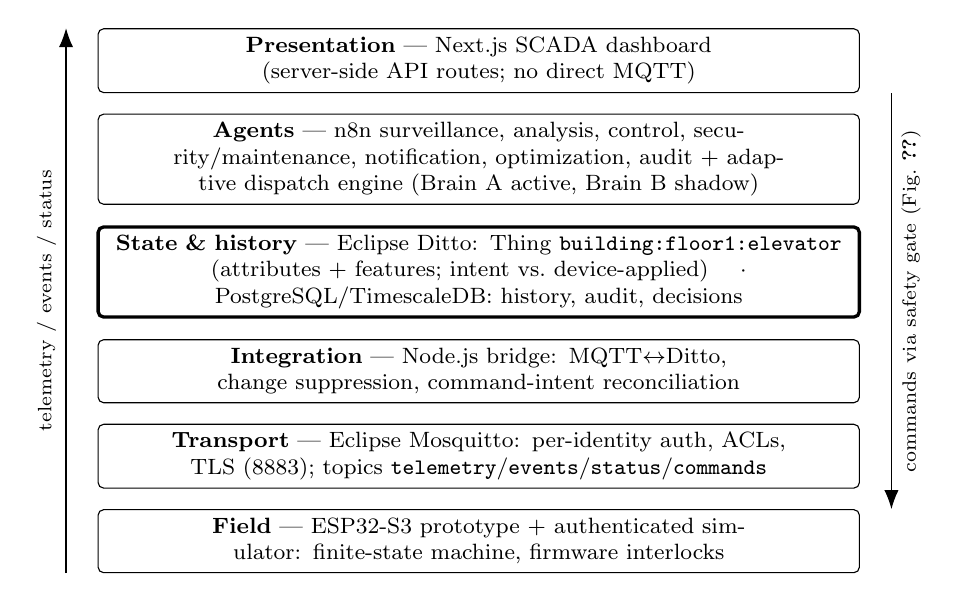
\begin{tikzpicture}[
  font=\footnotesize,
  band/.style={draw, rounded corners=2pt, text width=0.78\textwidth, align=center,
               minimum height=8mm, inner sep=3pt},
  node distance=2.6mm,
  >={Latex[length=2.4mm]},
]
\node[band] (pres) {\textbf{Presentation} --- Next.js SCADA dashboard (server-side API routes; no direct MQTT)};
\node[band, below=of pres] (agent) {\textbf{Agents} --- n8n surveillance, analysis, control, security/maintenance, notification, optimization, audit $+$ adaptive dispatch engine (Brain~A active, Brain~B shadow)};
\node[band, below=of agent, very thick] (state) {\textbf{State \& history} --- Eclipse Ditto: Thing \texttt{building:floor1:elevator} (attributes $+$ features; intent vs.\ device-applied) \quad$\cdot$\quad PostgreSQL/TimescaleDB: history, audit, decisions};
\node[band, below=of state] (integ) {\textbf{Integration} --- Node.js bridge: MQTT$\leftrightarrow$Ditto, change suppression, command-intent reconciliation};
\node[band, below=of integ] (trans) {\textbf{Transport} --- Eclipse Mosquitto: per-identity auth, ACLs, TLS (8883); topics \texttt{telemetry}/\texttt{events}/\texttt{status}/\texttt{commands}};
\node[band, below=of trans] (field) {\textbf{Field} --- ESP32-S3 prototype $+$ authenticated simulator: finite-state machine, firmware interlocks};
\draw[->] ([xshift=-4mm]field.south west) -- ([xshift=-4mm]pres.north west)
  node[midway, rotate=90, anchor=south, font=\scriptsize]{telemetry / events / status};
\draw[->] ([xshift=4mm]pres.south east) -- ([xshift=4mm]field.north east)
  node[midway, rotate=90, anchor=north, font=\scriptsize]{commands via safety gate (Fig.~\ref{fig:command-path})};
\end{tikzpicture}
\caption{Layered architecture. Telemetry flows up from the field to the state authority and its consumers; every command flows down only through the deterministic safety gate of Fig.~\ref{fig:command-path}. Eclipse Ditto, not the dashboard, is the operational source of truth.}
\label{fig:architecture}
\end{figure*}

The physical layer is a reduced-scale four-floor, single-cabin prototype controlled by ESP32-S3 firmware. The communication layer uses Mosquitto with JSON topics \topicbase\artifact{telemetry}, \topicbase\artifact{events}, \topicbase\artifact{status}, and \topicbase\artifact{commands}. The twin layer is Eclipse Ditto, accessed through \artifact{/api/2/things/\{thingId\}}. The history layer is PostgreSQL/TimescaleDB. The agent layer consists of n8n workflows and a dispatch engine. The presentation layer is the Next.js SCADA dashboard.

Table~\ref{tab:responsibility-boundaries} records the responsibility boundary that guided the implementation. This is a core design decision because failures in cyber-physical systems often arise when a layer quietly assumes authority that belongs elsewhere. The dashboard can request, but not execute. The bridge can forward accepted intent, but not decide safety. The workflow layer can analyze and route, but not override deterministic admission. The firmware remains responsible for local actuation checks even after backend admission.

\begin{table*}[t]
\caption{Responsibility boundaries in the implemented architecture}
\label{tab:responsibility-boundaries}
\centering
\footnotesize
\begin{tabularx}{\textwidth}{@{}p{0.17\textwidth}p{0.21\textwidth}Yp{0.18\textwidth}@{}}
\toprule
Layer & Owns & Must not own & Reliability/security rationale \\
\midrule
ESP32-S3 firmware & Local state machine, actuator control, emergency and movement interlocks, MQTT telemetry and command subscription. & Fleet history, operator identity, long-term analytics, or direct dashboard state. & Keeps immediate protection close to the physical process and allows safe local behavior during network loss. \\
MQTT broker & Authenticated message transport, topic routing, retained status, ACL enforcement. & Operational truth, UI state, or command authorization. & Avoids treating transient wire messages as the authoritative model. \\
Bridge & Telemetry normalization, Ditto feature writes, command-intent reconciliation, MQTT command forwarding. & Human authorization, risk acceptance, or hidden business logic. & Makes the bridge auditable and recoverable after restart; accepted intent can be reconciled from Ditto. \\
Eclipse Ditto & Current operational state, attributes, subsystem features, command intent, policy boundary. & Long-term history or direct motor execution. & Gives all consumers one source of truth while preserving device-side interlocks. \\
PostgreSQL/TimescaleDB & Telemetry history, audit, command decisions, notifications, maintenance and dispatch records. & Current operational authority. & Enables traceability and analytics without making stale database rows control the elevator. \\
n8n workflows & Surveillance, analysis, maintenance, security, notifications, audit routing, bounded command requests. & Safety-critical command admission or LLM-based authorization. & Enables agentic automation while keeping decisions inspectable and testable. \\
Next.js SCADA dashboard & Operator visualization, history views, command-request UI, server-side API calls. & Direct MQTT publication or client-side secrets. & Prevents browser bypass of Ditto, safety gate, and audit logging. \\
\bottomrule
\end{tabularx}
\end{table*}

\begin{figure*}[t]
\centering
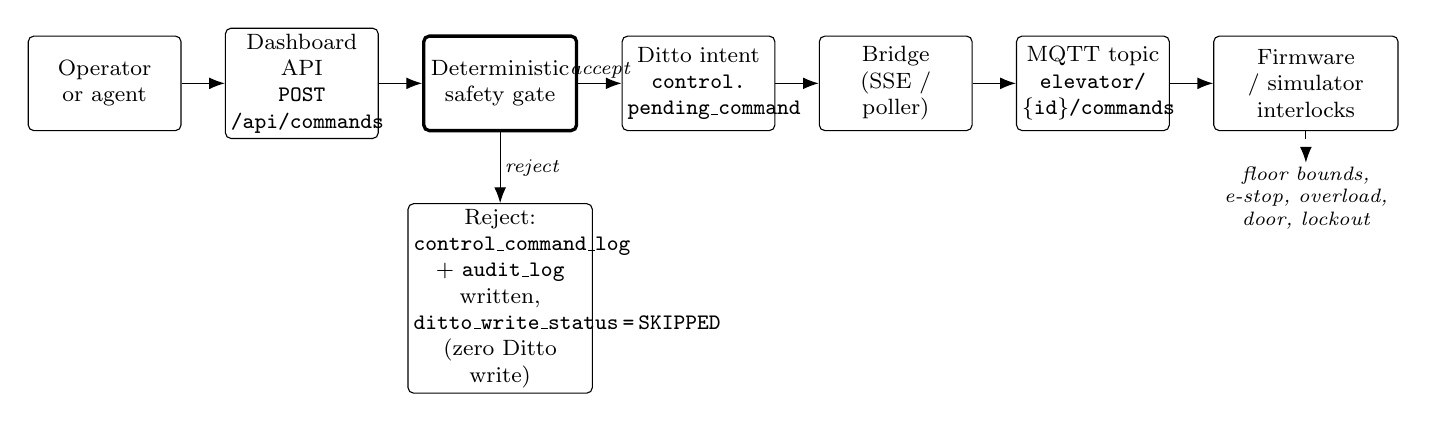
\begin{tikzpicture}[
  font=\footnotesize,
  >={Latex[length=2mm]},
  box/.style={draw, rounded corners=2pt, align=center, text width=18mm,
              minimum height=12mm, inner sep=2pt},
  gate/.style={box, very thick},
  term/.style={box, text width=22mm},
  lbl/.style={font=\scriptsize\itshape, inner sep=1.5pt},
  node distance=5.5mm and 5.5mm,
]
% main accept pipeline (left to right)
\node[box] (op) {Operator or agent};
\node[box, right=of op] (api) {Dashboard API\\\texttt{POST}\\\texttt{/api/commands}};
\node[gate, right=of api] (gate) {Deterministic\\safety gate};
\node[box, right=of gate] (ditto) {Ditto intent\\\texttt{control.}\\\texttt{pending\_command}};
\node[box, right=of ditto] (bridge) {Bridge\\(SSE / poller)};
\node[box, right=of bridge] (mqtt) {MQTT topic\\\texttt{elevator/}\\\texttt{\{id\}/commands}};
\node[term, right=of mqtt] (dev) {Firmware / simulator interlocks};
\draw[->] (op) -- (api);
\draw[->] (api) -- (gate);
\draw[->] (gate) -- node[above, lbl] {accept} (ditto);
\draw[->] (ditto) -- (bridge);
\draw[->] (bridge) -- (mqtt);
\draw[->] (mqtt) -- (dev);
% reject branch (downward from the gate)
\node[term, below=9mm of gate] (reject)
  {Reject: \texttt{control\_command\_log} $+$ \texttt{audit\_log} written,\\
   \texttt{ditto\_write\_status\,=\,SKIPPED} (zero Ditto write)};
\draw[->] (gate) -- node[right, lbl] {reject} (reject);
% interlock note under device
\node[lbl, below=4mm of dev, text width=24mm, align=center] (lock)
  {floor bounds, e-stop, overload, door, lockout};
\draw[->, dashed] (dev) -- (lock);
\end{tikzpicture}
\caption{Safety-gated command path. The browser, workflows, and optional LLM never publish device commands directly. Accepted intent is persisted as Ditto command intent and forwarded by the bridge; rejected commands are logged for audit but produce zero Ditto writes (\texttt{ditto\_write\_status\,=\,SKIPPED}). The firmware or simulator applies local interlocks before actuation.}
\label{fig:command-path}
\end{figure*}

\subsection{Command Authority Principle}

Fig.~\ref{fig:command-path} is the architectural centerpiece. The dashboard and n8n workflows may request commands. The deterministic gate decides whether they can become Ditto intent. The bridge forwards only accepted, fresh, non-duplicate command intents. The firmware or simulator remains the last software boundary before actuation. This design prevents three unsafe shortcuts: browser-to-MQTT command publication, LLM-generated command authorization, and direct workflow mutation of actuator state.

\subsection{Agentic Automation Boundary}

The n8n layer is decomposed into specialized workflows. The surveillance agent canonicalizes twin events and records timelines. The analysis agent computes deterministic risk flags and optional human-readable explanation. The control agent applies the safety gate. Security and maintenance agents update security state and work orders. Notification agents write and deliver outbox records. Optimization and audit agents record dispatch decisions and operational traces. This is a multi-workflow agentic system, but the authority boundary is conservative: risk classification, command admission, and dispatch policy selection are deterministic and auditable.

Table~\ref{tab:agent-workflows} summarizes the workflow roles. The important point is not the number of workflows, but the fact that each workflow has a bounded contract and produces explicit state or audit artifacts. In particular, the analysis workflow may attach an LLM-generated explanation when the local model is enabled, but the command gate does not read that explanation as an authorization signal.

\begin{table*}[t]
\caption{Bounded agentic workflow decomposition}
\label{tab:agent-workflows}
\centering
\footnotesize
\begin{tabularx}{\textwidth}{@{}p{0.18\textwidth}p{0.18\textwidth}Yp{0.18\textwidth}@{}}
\toprule
Workflow role & Trigger & Decision/action & Evidence or state written \\
\midrule
Surveillance agent & Ditto change, MQTT-derived twin event, scheduled scan. & Canonicalize event, deduplicate, update timeline, preserve correlation identifiers. & Telemetry/history rows and normalized event envelope. \\
Analysis agent & New telemetry/risk event. & Apply deterministic risk rules; optionally request explanatory text from local LLM. & \artifact{ai\_analysis} feature, risk flags, audit rows. \\
Control agent & Operator or workflow command request. & Run deterministic command safety gate and branch accepted/rejected paths. & \artifact{control\_command\_log}, \artifact{audit\_log}, Ditto writes only if accepted. \\
Security agent & RFID/security/forced-door event or risk escalation. & Update security state, request lockdown only through the gate, surface human-review requirement. & \artifact{security} feature and audit rows. \\
Maintenance agent & Wear/risk threshold, repeated incident, scheduled review. & Create or update work-order state using rule-based evidence. & \artifact{maintenance\_schedule}, \artifact{maintenance\_work\_orders}. \\
Notification agent & Alert or outbox due event. & Build dedupe key, select channels, retry or mark failed/sent. & \artifact{notification\_outbox}. \\
Optimization/audit agent & Dispatch cycle or audit event. & Record dispatch decisions, policy changes, reward/proxy outcomes, workflow activity. & Dispatch/audit tables and dashboard history APIs. \\
\bottomrule
\end{tabularx}
\end{table*}

\section{Implementation}

\subsection{Prototype and Firmware}

Table~\ref{tab:prototype-specs} summarizes the physical prototype, shown in Fig.~\ref{fig:prototype}. The ESP32-S3 was selected for Wi-Fi connectivity, GPIO, ADC, SPI/I2C, timers, PWM-capable pins, and sufficient memory for MQTT/TLS operation in a laboratory prototype \cite{espressifEsp32S3Datasheet,espidfMqttClient}.

\begin{figure}[t]
\centering
% TODO(human): confirm permission to publish this prototype photograph.
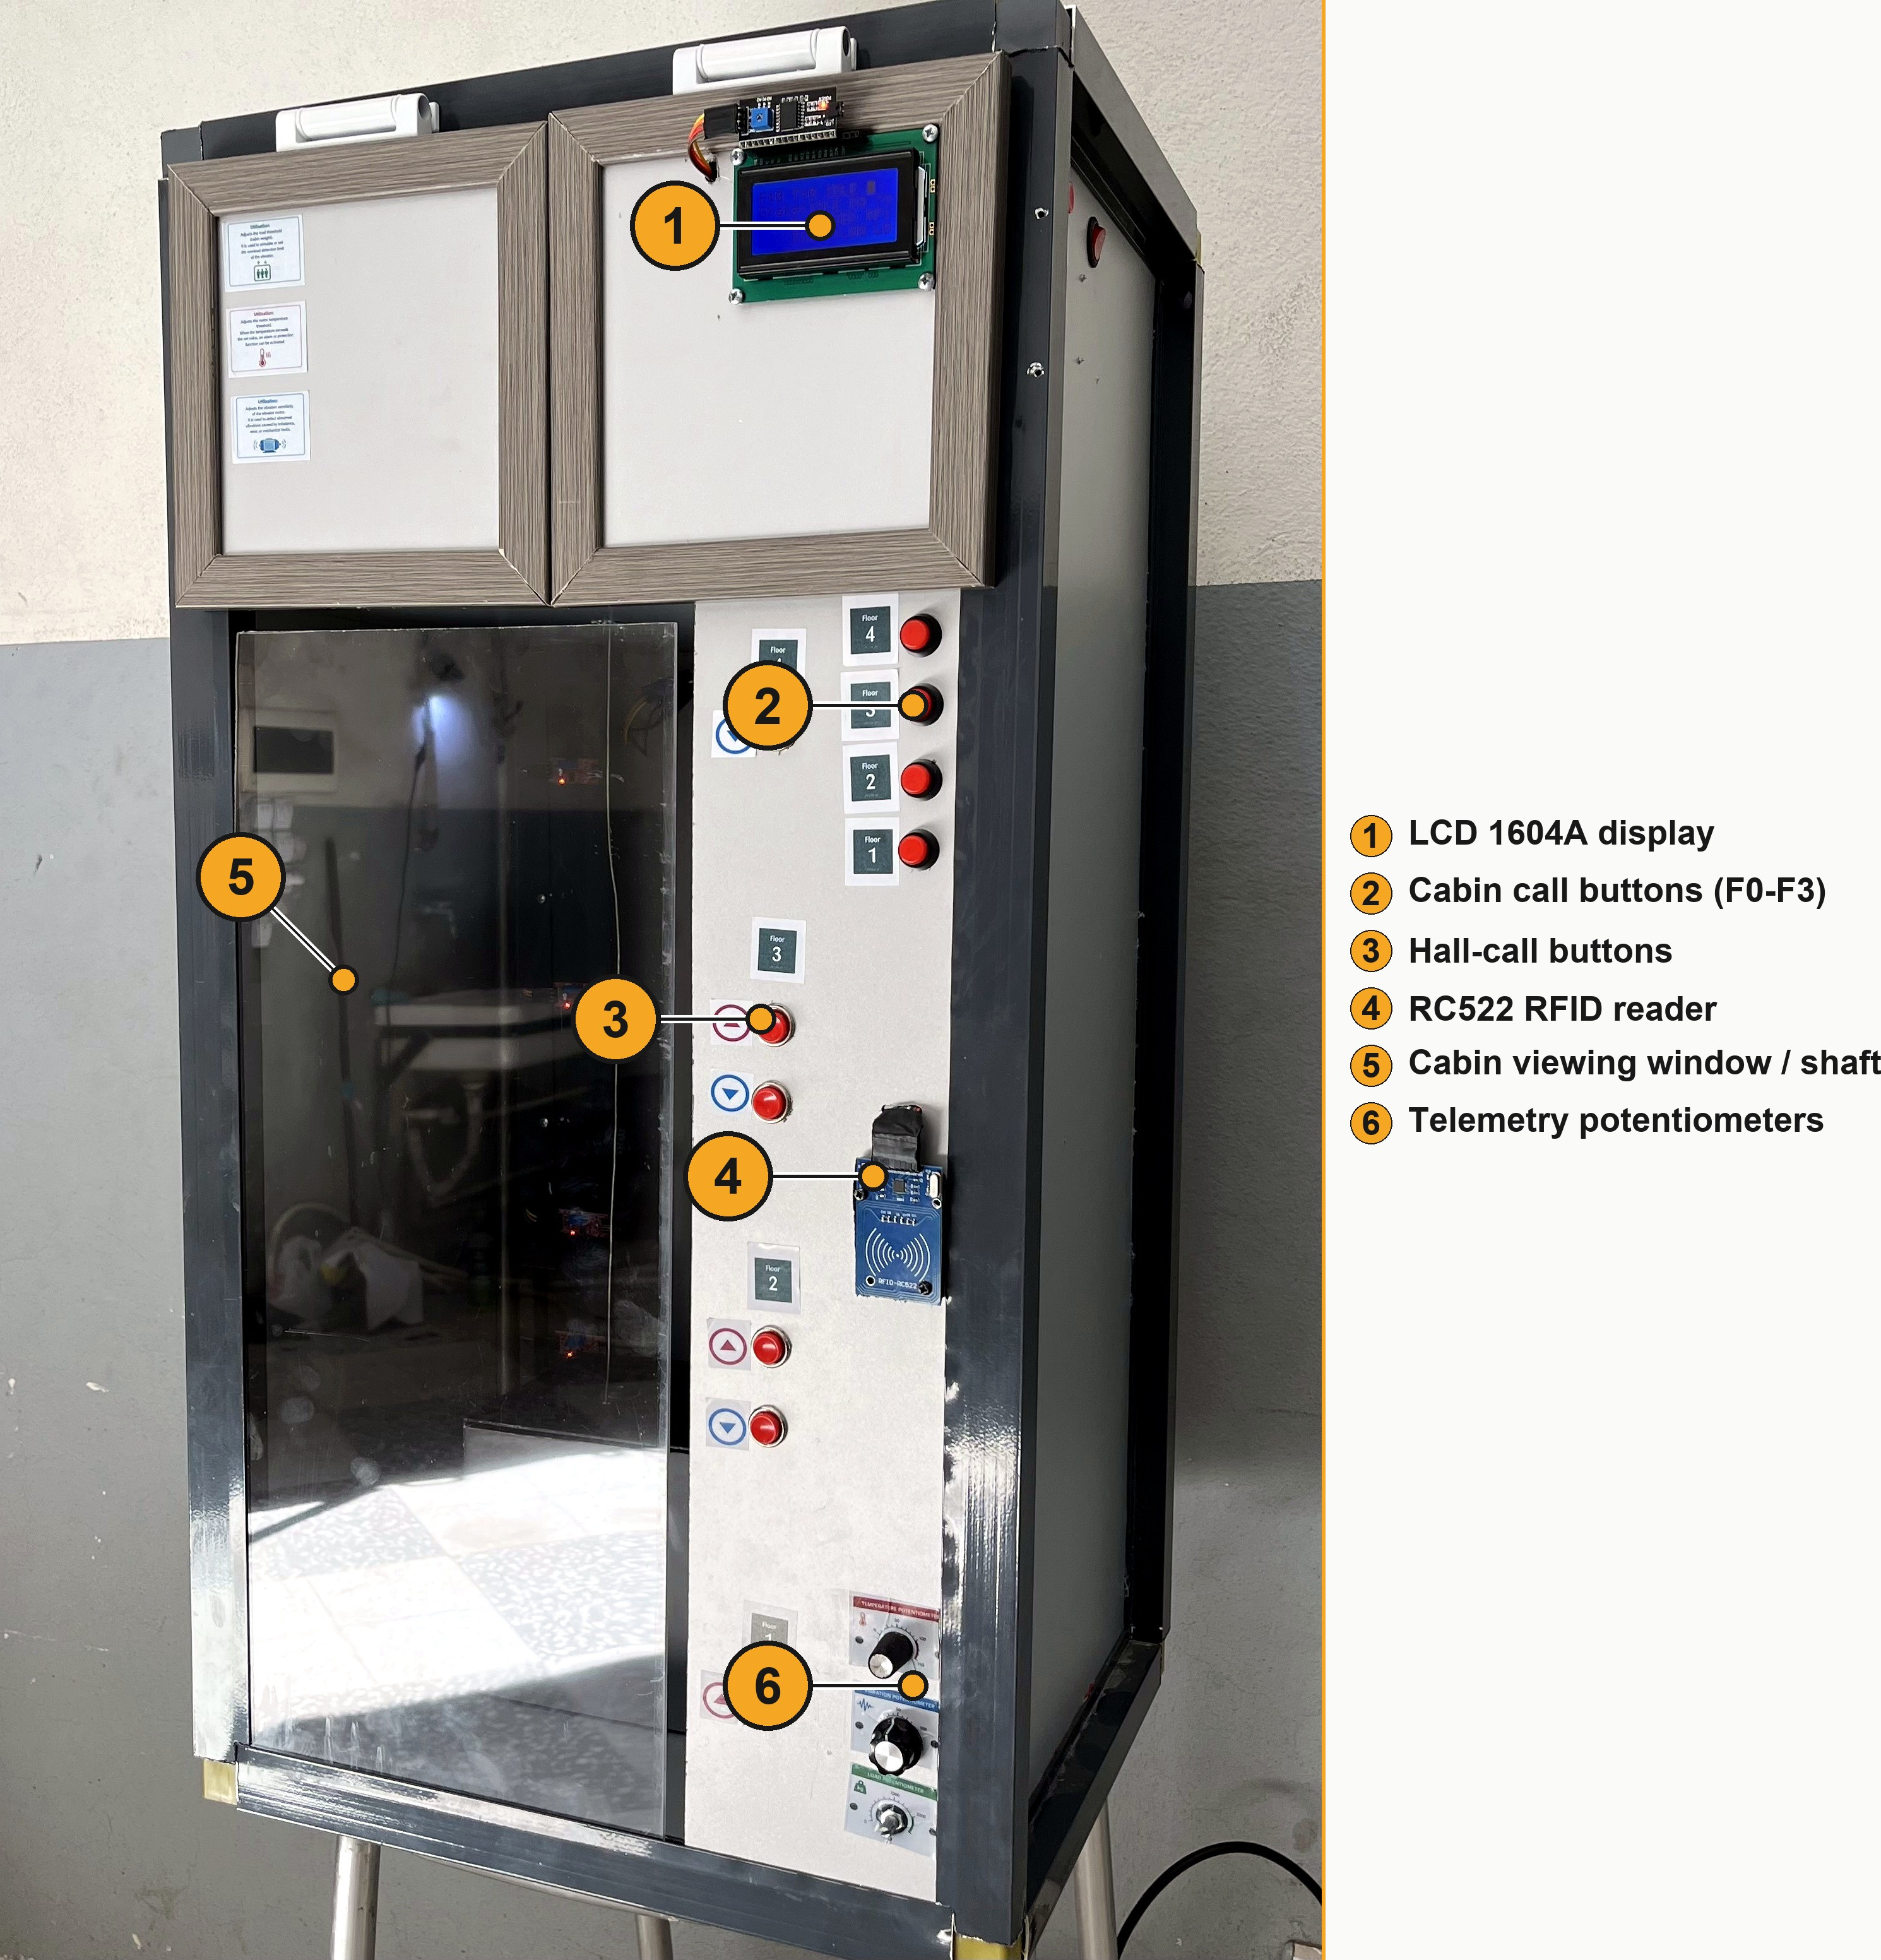
\includegraphics[width=0.92\columnwidth]{prototype.jpg}
\caption{Reduced-scale four-floor, single-cabin ESP32-S3 elevator prototype (annotated). Temperature, vibration, and load are simulated through ADC potentiometers; KY-024 and SPDT switches are mounted provisions only, not validated in the deployed firmware. \textit{Pending author permission to publish.}}
\label{fig:prototype}
\end{figure} The deployed firmware implements a finite-state machine with idle, door-opening, door-wait, door-closing, moving-up, moving-down, arrival, error-stop, and emergency states. Remote commands are not direct GPIO operations; they are parsed into state-machine requests and checked against firmware-side interlocks.

\begin{table}[t]
\caption{Reduced-scale elevator prototype characteristics}
\label{tab:prototype-specs}
\centering
\footnotesize
\begin{tabularx}{\columnwidth}{@{}p{0.34\columnwidth}Y@{}}
\toprule
Item & Value or evidence boundary \\
\midrule
Physical configuration & One cabin, four logical floors numbered 0--3. \\
Frame dimensions & Approximately 84 cm high, 44 cm wide, 38 cm deep. \\
Cabin dimensions & 15 cm cube, approximately 3375 cm$^3$. \\
Movement timing & Approximately 6 s per adjacent floor, author-recorded prototype timing, not instrumented video/log evidence. \\
Controller & ESP32-S3 microcontroller running the custom elevator firmware. \\
Cabin motion & NEMA17 stepper through microstep driver; calibrated step-count profile; KY-024 Hall sensors mounted for future confirmation. \\
Door motion & DC motor through L298N/HW-095 H-bridge; timed travel profile; SPDT limit switches mounted for future confirmation. \\
Local HMI & 16x4 I2C LCD, push buttons, emergency input, buzzer, fan relay. \\
Security input & MFRC522 RFID support in firmware; physical UID scan evidence is outside current validation scope. \\
Safety telemetry & Temperature, vibration, and load currently simulated through ADC potentiometers. \\
\bottomrule
\end{tabularx}
\end{table}

The firmware publishes JSON telemetry to \artifact{elevator/\mqttid/telemetry}, events to \artifact{elevator/\mqttid/events}, retained status to \artifact{elevator/\mqttid/status}, and subscribes to \artifact{elevator/\mqttid/commands}. Firmware telemetry uses a Ditto-aligned feature envelope, and the repository configuration sets a 3000 ms periodic telemetry interval when not moving, a 5000 ms status interval, and position-oriented updates during motion. These are configured design parameters unless instrumented captures are added.

\subsection{MQTT Security Baseline}

The broker disables anonymous access and uses per-client identities: \artifact{esp32-elevator}, \artifact{bridge}, \artifact{agents}, \artifact{dashboard}, and \artifact{healthcheck}. The ESP32 identity publishes only its telemetry, events, and status and subscribes only to its commands. The dashboard identity is read-only for diagnostics and cannot publish command topics. The bridge identity can publish device commands after Ditto intent is accepted. The security evidence package shows anonymous and wrong-password connections rejected with \artifact{not authorised}, while an authenticated bridge subscriber received telemetry. A separate field TLS evidence capture on port 8883 confirms successful publish/subscribe over the ESP32-side TLS listener; the steady-state TLS round-trip time was measured separately on a loopback broker (Section~\ref{sec:eval}).

The topic convention is deliberately narrow. Periodic telemetry carries feature-shaped JSON snapshots; events carry discrete safety, security, and maintenance incidents; status carries retained presence; and commands are cloud-to-device messages produced only by authorized backend identities. This separation allows ACLs to express operational authority: an ESP32 credential can never publish commands, and a dashboard credential can never bypass the server-side command API. In a multi-building deployment, the same convention extends through Thing IDs and MQTT-safe identifiers without changing the UI control model.

\subsection{MQTT-to-Ditto Bridge}

The Node.js bridge subscribes to \artifact{elevator/+/telemetry}, \artifact{elevator/+/events}, and \artifact{elevator/+/status}, parses JSON, resolves the Thing ID, maps aliases to canonical field names, groups values into Ditto features, suppresses unchanged writes, retries Ditto writes, and updates microcontroller presence. It writes specific feature paths under \artifact{/api/2/things/\{thingId\}} rather than replacing the full Thing document.

The reverse path is implemented through Ditto Server-Sent Events plus a polling recovery path for \artifact{features/control/properties/pending\_command}. The bridge filters stale, duplicate, rejected, or already-forwarded commands. Accepted intents are translated to compact MQTT commands such as \artifact{MOVE\_TO\_FLOOR}, \artifact{EMERGENCY\_STOP}, \artifact{RESET}, and \artifact{DISPATCH\_POLICY}.

\subsection{Ditto Thing Model and Persistence}

The default Thing ID is \thingid, mapped to MQTT-safe ID \mqttid. Attributes store metadata and fleet-level status, while features represent subsystems such as \artifact{cabin}, \artifact{door}, \artifact{motor}, \artifact{security}, \artifact{fan}, \artifact{microcontroller}, \artifact{control}, \artifact{energy}, \artifact{performance}, \artifact{ai\_analysis}, \artifact{predicted\_failures}, and \artifact{maintenance\_schedule} (Fig.~\ref{fig:ditto-model}). The \artifact{control} feature separates command intent from device-applied state. For dispatch, \artifact{control.dispatch\_policy} is the authoritative intent selected by the engine, while \artifact{control.device\_applied\_policy} is reported by the firmware or simulator.

\begin{figure}[t]
\centering
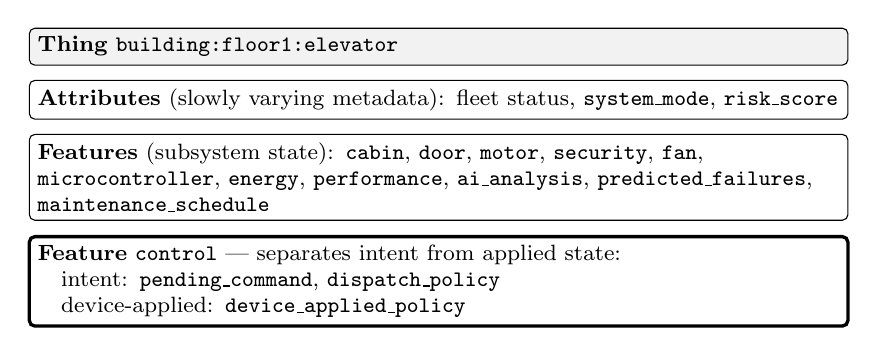
\begin{tikzpicture}[font=\footnotesize,
  blk/.style={draw, rounded corners=2pt, align=left, inner sep=3pt, text width=0.84\columnwidth},
  node distance=1.8mm,
]
\node[blk, fill=black!5] (thing) {\textbf{Thing} \texttt{building:floor1:elevator}};
\node[blk, below=of thing] (attr) {\textbf{Attributes} (slowly varying metadata): fleet status, \texttt{system\_mode}, \texttt{risk\_score}};
\node[blk, below=of attr] (feat) {\textbf{Features} (subsystem state): \texttt{cabin}, \texttt{door}, \texttt{motor}, \texttt{security}, \texttt{fan}, \texttt{microcontroller}, \texttt{energy}, \texttt{performance}, \texttt{ai\_analysis}, \texttt{predicted\_failures}, \texttt{maintenance\_schedule}};
\node[blk, below=of feat, very thick] (ctrl) {\textbf{Feature} \texttt{control} --- separates intent from applied state:\\
\hspace*{1em}intent: \texttt{pending\_command}, \texttt{dispatch\_policy}\\
\hspace*{1em}device-applied: \texttt{device\_applied\_policy}};
\end{tikzpicture}
\caption{Eclipse Ditto Thing model. Attributes hold slowly varying metadata; features hold subsystem state. The \texttt{control} feature explicitly separates command \emph{intent} from \emph{device-applied} state---the property that lets a rejected command leave the twin unchanged.}
\label{fig:ditto-model}
\end{figure}

PostgreSQL/TimescaleDB stores raw telemetry, audit events, command decisions, notifications, maintenance work orders, system health records, and dispatch decisions. The final evidence export records seven application tables and 19,901 rows in \artifact{telemetry\_raw} as of 2026-06-13 02:07:12.

The use of both Ditto and PostgreSQL is intentional. Ditto answers ``what is the asset state now?'' and PostgreSQL answers ``what happened, why, when, and who requested it?'' A rejected command is therefore just as important as an accepted command: it proves that the system constrained an unsafe or unauthorized request and preserved the reason for later audit. This separation also supports future retention policies, fleet analytics, and incident reconstruction without overloading the twin with historical arrays.

\subsection{Safety Gate}

The command safety gate is implemented in the shared JavaScript package and mirrored in the n8n control workflow. It validates command allow-list, required fields, source, source agent, reason, confirmation, system mode, emergency stop, door state, overload, forced entry, risk threshold, target floor bounds, twin freshness, duplicate cooldown, dispatch-policy validity, and Ditto availability. If any mandatory predicate fails, the decision is persisted as rejected, \artifact{ditto\_write\_status} is \artifact{SKIPPED}, and the planned Ditto write list is empty.

\begin{equation}
\label{eq:gate}
\begin{aligned}
\operatorname{accept}(c,T) ={}& \operatorname{allowlisted}(c) \wedge \operatorname{valid}(c) \\
&{}\wedge \operatorname{authorized}(c) \wedge \operatorname{fresh}(T) \\
&{}\wedge \operatorname{safeMode}(T) \wedge \operatorname{safeInterlocks}(T) \\
&{}\wedge \operatorname{riskWithinLimit}(c,T) \wedge \operatorname{dittoReachable}(T).
\end{aligned}
\end{equation}

Here $c$ is the requested command and $T$ the current twin snapshot. The predicates correspond directly to the checks above: $\operatorname{allowlisted}$ and $\operatorname{valid}$ test the command catalog and required fields; $\operatorname{authorized}$ tests source, source agent, reason, and human confirmation; $\operatorname{fresh}$ requires a recent twin; $\operatorname{safeMode}$ excludes unsafe system modes; $\operatorname{safeInterlocks}$ tests emergency stop, door state, overload, and forced entry; $\operatorname{riskWithinLimit}$ bounds the risk score and target-floor range; and $\operatorname{dittoReachable}$ requires the twin store to be writable. A command is admitted only if all predicates hold; the implementation records all failing predicates rather than returning only the first failure.

Table~\ref{tab:gate-rules} lists the principal rule families. The final software evidence confirms that rejected decisions carry no Ditto writes. In the live command-path run, this property was not only unit-tested but also observed in database rows: every rejected command had \artifact{ditto\_write\_status = SKIPPED}.

\begin{table*}[t]
\caption{Deterministic command safety-gate rule families}
\label{tab:gate-rules}
\centering
\footnotesize
\begin{tabularx}{\textwidth}{@{}p{0.18\textwidth}p{0.28\textwidth}Y@{}}
\toprule
Rule family & Examples & Safety effect \\
\midrule
Command catalog & Unknown commands; unsupported aliases; missing required fields. & Prevents arbitrary payloads from becoming Ditto writes or device commands. \\
Source and accountability & Source must be authorized; source agent must be explicit; operator reason may be required. & Preserves traceability and blocks anonymous automation paths. \\
Human confirmation & Emergency stop, reset, lockdown, release, maintenance-mode transitions. & Prevents accidental state-changing actions and forces explicit operator intent. \\
Twin freshness and availability & Stale twin; Ditto unavailable; missing safety snapshot. & Avoids acting on old or incomplete operational state. \\
Safety interlocks & Emergency stop, overload, door open, forced entry, critical risk, unsafe system mode. & Blocks movement and unsafe recovery commands before they reach the device. \\
Bounds and policy validity & Target floor outside 0--3; unknown dispatch policy; invalid policy parameters. & Preserves physical and logical limits of the prototype. \\
Duplicate/cooldown & Same command, same target, same source within cooldown window. & Reduces repeated operator clicks or workflow churn. \\
Zero-write invariant & Any rejection clears the planned write array. & Ensures rejected commands cannot partially mutate Ditto state. \\
\bottomrule
\end{tabularx}
\end{table*}

\subsection{Adaptive Dispatch Engine}

The dispatch policy engine chooses the operating policy, not direct movement commands. Policies include \artifact{SCAN\_COLLECTIVE}, \artifact{UP\_PEAK}, \artifact{DOWN\_PEAK}, \artifact{ECO\_ENERGY}, \artifact{NEAREST\_GREEDY}, \artifact{HEALTH\_LIMP}, \artifact{BALANCED\_INTERFLOOR}, and \artifact{SECURITY\_RESTRICTED}. Hard safety overrides such as \artifact{EMERGENCY\_STOP}, \artifact{OVERLOAD\_HOLD}, \artifact{FULL\_LOCKDOWN}, and \artifact{FIRE\_RECALL} pre-empt optimization.

Brain A is the active deterministic scorer. Brain B is a softmax linear challenger over the shared feature vector. Brain B is logged in shadow mode and cannot become authoritative unless future evidence satisfies promotion gates and a human approves. This separation preserves explainability, rollback, and safety authority.

Table~\ref{tab:dispatch-policies} summarizes the policy layer. These policies select dispatch behavior, not immediate cabin actuation. A policy command still goes through the same safety gate and is then reported separately as intent and applied state.

\begin{table}[t]
\caption{Dispatch policies and safety overrides}
\label{tab:dispatch-policies}
\centering
\footnotesize
\begin{tabularx}{\columnwidth}{@{}p{0.38\columnwidth}Y@{}}
\toprule
Policy or override & Role \\
\midrule
\artifact{SCAN\_COLLECTIVE} & Default collective service policy. \\
\artifact{UP\_PEAK} / \artifact{DOWN\_PEAK} & Traffic-biased policies for directional demand. \\
\artifact{ECO\_ENERGY} & Energy-saving policy when demand and fairness conditions allow it. \\
\artifact{NEAREST\_GREEDY} & Short-horizon nearest-call service for sparse demand. \\
\artifact{HEALTH\_LIMP} & Reduced-stress operation under degraded machine indicators. \\
\artifact{BALANCED\_INTERFLOOR} & General balanced policy for mixed traffic. \\
\artifact{SECURITY\_RESTRICTED} & Restricted service under elevated security state. \\
\artifact{FIRE\_RECALL}, \artifact{EMERGENCY\_STOP}, \artifact{FULL\_LOCKDOWN}, \artifact{OVERLOAD\_HOLD} & Hard safety overrides that pre-empt optimization. \\
\bottomrule
\end{tabularx}
\end{table}

\subsection{SCADA Dashboard}

The Next.js dashboard reads Ditto through server-side APIs and history routes (Fig.~\ref{fig:dashboard}). Dynamic values are handled in client hooks to avoid SSR hydration errors. The dashboard command center posts to \artifact{/api/commands}; it does not publish MQTT commands. This preserves separation between UI, logic, state, and device transport.

\begin{figure}[t]
\centering
% TODO(human): confirm permission to publish this dashboard screenshot.
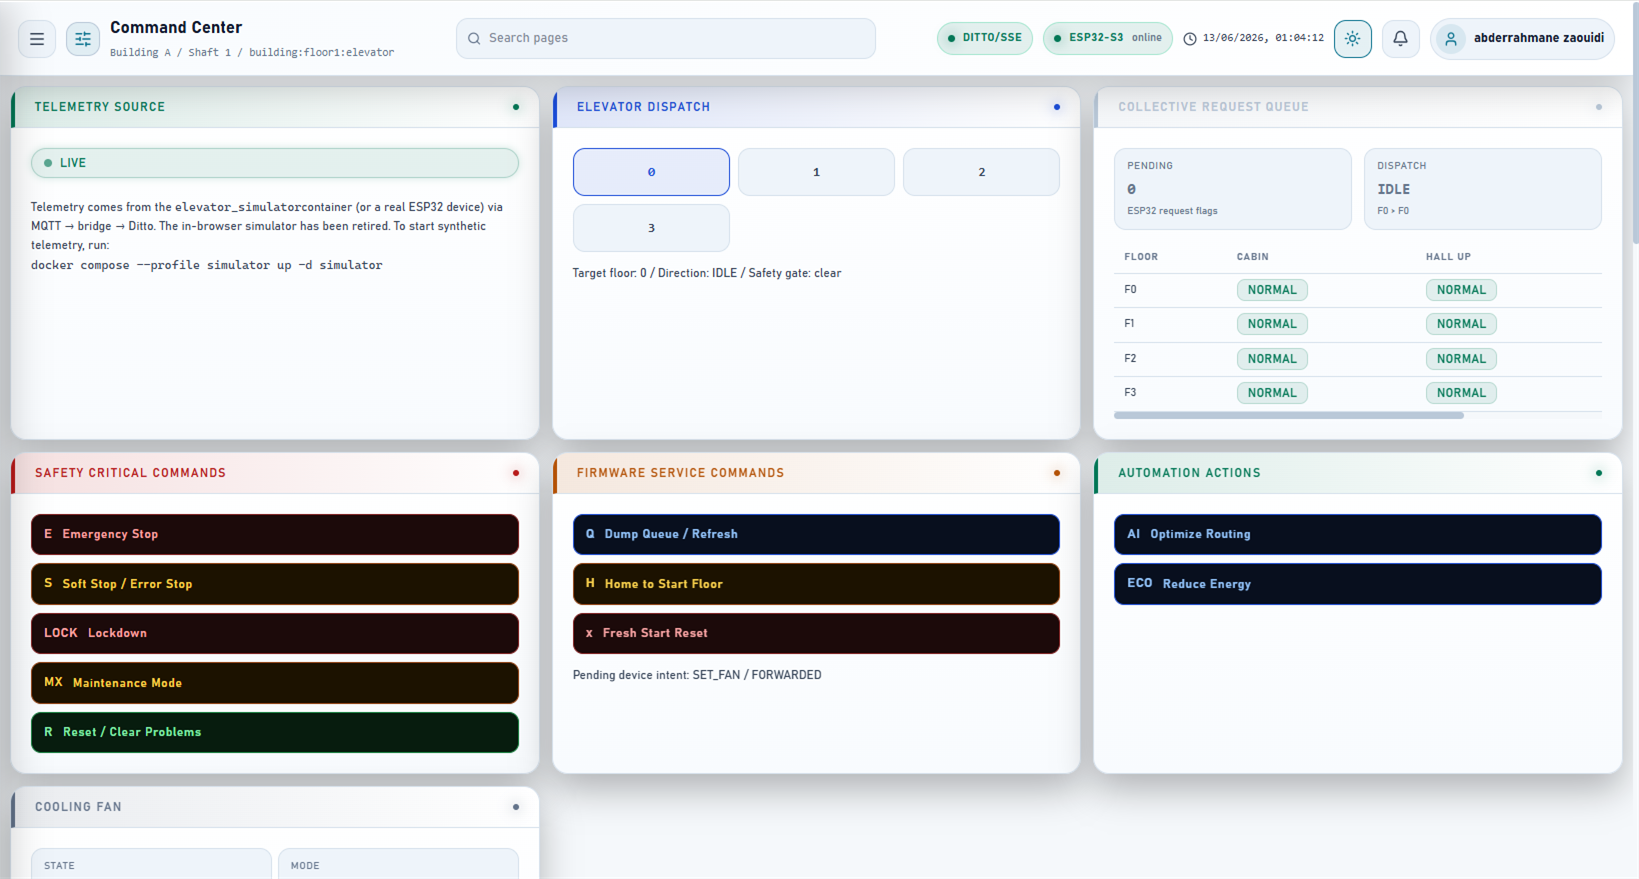
\includegraphics[width=\columnwidth]{dashboard_command_center.png}
\caption{SCADA command center. Operator commands post to \artifact{/api/commands} and pass the deterministic safety gate; recent command decisions and their accept/reject reasons are shown. \textit{Pending author permission to publish.}}
\label{fig:dashboard}
\end{figure}

The dashboard is therefore not a thin MQTT client. Its pages surface the live twin, historical telemetry, risk analysis, maintenance state, security state, command decisions, and dispatch policy. The server-side routes hide Ditto and database credentials from the browser and make the command path uniform for operator and workflow-originated requests. The current authentication boundary is prototype-level; production hardening requires server-side sessions, OIDC or equivalent identity management, role-based access control, HTTPS, and audit-linked user identities.

\section{Validation and Evaluation}
\label{sec:eval}

\subsection{Evidence Policy}

Validation uses an evidence boundary rather than a blanket PASS claim. A result is marked PASS only when a repository artifact, exported log, screenshot, query output, or command transcript exists. Software tests validate software logic and integration. Documented hardware integration records the built prototype, wiring, dimensions, and observed behavior, but it is not equivalent to certified or instrumented physical validation.

\subsection{Validation Summary}

Table~\ref{tab:validation-summary} summarizes the validated artifacts. The final live software run was executed on 2026-06-13 against the full Docker stack, the dashboard, Ditto, TimescaleDB, n8n, bridge, Mosquitto with authentication and ACLs, and an authenticated ESP32-compatible simulator.

The campaign intentionally uses qualified statuses. ``PASS'' is reserved for procedures with captured evidence and expected behavior. ``Software PASS'' describes logic and integration proven by automated tests, logs, exports, or live-stack traces. ``Documented integration'' describes physical build evidence without a separate measurement campaign. ``Outside current scope'' marks work that must not be implied by simulator or configuration evidence. This vocabulary keeps the evaluation honest while still showing that the software architecture is reproducible.

\begin{table*}[t]
\caption{Validation evidence summary}
\label{tab:validation-summary}
\centering
\footnotesize
\begin{tabularx}{\textwidth}{@{}p{0.22\textwidth}p{0.18\textwidth}Yp{0.16\textwidth}@{}}
\toprule
Subsystem & Status & Evidence & Boundary \\
\midrule
MQTT topic convention & PASS & \artifact{evidence/mqtt/topic\_validator\_output.txt}: scanned 266 files, no unexpected legacy topic patterns, expected canonical topics present. & Software/configuration evidence. \\
MQTT authentication and ACLs & PASS & \artifact{acl\_security\_tests.txt}: anonymous and wrong-password connections denied; authenticated bridge subscriber received telemetry. & Broker-side evidence. \\
TLS publish/subscribe & PASS & Workspace \artifact{evidence/mqtt/05-roundtrip-tls.txt}: TLS publish exit 0 and subscriber receive exit 0 on 8883. & Field RTT not timed; loopback RTT in Table~\ref{tab:metrics}. \\
Bridge and Ditto sync & PASS & \artifact{bridge\_logs.txt} and Ditto Thing export show twin merges, online status, command-intent forwarding. & Software-stack evidence. \\
Command safety gate & PASS & \artifact{command\_safety\_gate\_test\_output.txt}: 33/33 assertions; live command rows show rejected commands with \artifact{SKIPPED} writes. & Deterministic software gate. \\
Dispatch engine & PASS & 61/61 dispatch assertions across policy, safety, orchestrator, Brain B, and evaluation suites. & Brain B remains shadow-only. \\
Simulator regression & PASS & \artifact{simulator\_pytest\_output.txt}: 33/33 pytest items in 0.31 s. & Simulator software evidence, not physical hardware proof. \\
Database/history & PASS & Seven application tables; \artifact{telemetry\_raw} count 19,901 rows on 2026-06-13. & Live database export. \\
End-to-end command path & PASS & Nine command-log rows; emergency stop, reset, rejected move, rejected invalid dispatch policy, accepted dispatch policy. & Device endpoint was authenticated simulator for final software run. \\
Physical prototype & Documented integration & Thesis photographs, dimensions, wiring, and author-recorded adjacent-floor timing of approximately 6 s. & Not certified; not fully instrumented. \\
\bottomrule
\end{tabularx}
\end{table*}

\subsection{Command-Path Results}

The final command-path transcript records nine live command decisions. An \artifact{EMERGENCY\_STOP} without confirmation was rejected. A confirmed \artifact{EMERGENCY\_STOP} was accepted and forwarded. A \artifact{MOVE\_TO\_FLOOR} request during unsafe state was rejected. \artifact{RESET\_EMERGENCY} was accepted. Unknown dispatch policies were rejected. Valid \artifact{SET\_DISPATCH\_POLICY} commands were accepted and adopted by the simulator. Every rejected command carried \artifact{ditto\_write\_status = SKIPPED}, demonstrating the zero-write invariant on live infrastructure.

\subsection{Quantitative Evidence}

Table~\ref{tab:metrics} separates measured software results, configured design parameters, and metrics deferred to future work. The distinction matters because configured intervals and the deterministic decision-time microbenchmarks reported below are useful evidence but are not substitutes for instrumented end-to-end latency, which remains future work.

\begin{table*}[t]
\caption{Quantitative evidence inventory: measured, configured, and future-work metrics}
\label{tab:metrics}
\centering
\footnotesize
\begin{tabularx}{\textwidth}{@{}p{0.22\textwidth}Yp{0.20\textwidth}@{}}
\toprule
Metric & Current value and interpretation & Classification \\
\midrule
Adjacent-floor travel time & Approximately 6 s per floor; author-recorded prototype timing from the running reduced-scale rig, not instrumented. & Documented (author-recorded); instrumented timing is future work. \\
Telemetry publish interval & 3000 ms when not moving (firmware constant; simulator tick log 3.00 s). & Configured. \\
Status heartbeat & 5000 ms; bridge offline threshold 15000 ms. & Configured. \\
Bridge write interval & 1000 ms; command-intent poll interval 500 ms. & Configured. \\
Command safety-gate validation & 33/33 assertions; rejected commands carry zero Ditto writes. Suite duration is test-runner time, not latency. & Measured (functional). \\
Dispatch validation & 61/61 assertions across policy, safety, orchestrator, Brain~B, and evaluation suites. & Measured (functional). \\
Simulator regression & 33/33 pytest items. & Measured (functional). \\
MQTT round-trip time & Loopback steady-state (QoS 1, 500 samples): local broker median 1.11~ms, TLS listener median 1.19~ms; plus functional TLS publish/subscribe (exit 0) on port 8883. & Measured. \\
Safety-gate decision time & Median 5.7~$\mu$s for an accepted command, 4.4--5.6~$\mu$s for rejected classes; p99 below 20~$\mu$s (20{,}000 samples/class). & Measured (in-process). \\
Live dispatch decision time & Active Brain~A: median 9.5~$\mu$s (scorer) and 15.6~$\mu$s including context build; full orchestrator loop 22.4~$\mu$s. & Measured (in-process). \\
Cost of safety & Deterministic admission adds a median 5.3~$\mu$s of in-process computation over a direct dashboard$\rightarrow$MQTT serialization (0.42~$\mu$s). & Measured (in-process). \\
End-to-end command latency & Coarse transcript indicates sub-second for one dispatch restore; no paired timestamps. & Future work. \\
Ditto synchronization delay & Bridge logs show repeated twin merges and online status; no paired timestamps. & Future work. \\
Reconnection time & Reconnect logic present; no timed fault-injection capture. & Future work. \\
ESP32 resource usage & No heap, CPU, or loop-timing capture (requires the physical board). & Future work (hardware). \\
\bottomrule
\end{tabularx}
\end{table*}

The deterministic decision paths were microbenchmarked in-process over 20{,}000 samples per class on a single host, with per-call timing from \artifact{process.hrtime}; the raw distribution is archived in \artifact{evidence/perf/decision-latency.json}. The safety gate evaluates an accepted command in a median of 5.7~$\mu$s and a rejected command in 4.4--5.6~$\mu$s, with the 99th percentile below 20~$\mu$s. The active Brain~A dispatch decision takes a median of 15.6~$\mu$s from the twin snapshot, and the full orchestrator loop---context construction, decision, gate preview, and command assembly---completes in a median of 22.4~$\mu$s. These are CPU times of the decision logic, distinct from the test-suite durations reported by the runner, and they must not be read as end-to-end command latency, which additionally crosses the network, Ditto, and the device and remains future work. The deterministic admission adds only about 5.3~$\mu$s of computation per command relative to a direct dashboard-to-MQTT serialization: the cost of the safety discipline is architectural rather than a measurable performance penalty. Transport latency was measured separately over a loopback broker (\artifact{evidence/perf/mqtt-rtt.txt}): the steady-state MQTT round-trip is a median of 1.11~ms on the plain listener and 1.19~ms over the TLS listener (QoS~1, 500 samples each), confirming that the encrypted hop adds negligible per-message overhead once the handshake is established.

\begin{figure}[t]
\centering
\begin{tikzpicture}
\begin{axis}[
  width=\columnwidth, height=4.8cm,
  xlabel={Safety-gate decision time ($\mu$s)},
  ylabel={cumulative fraction},
  xmin=5, xmax=25, ymin=0, ymax=1,
  ytick={0,0.25,0.5,0.75,0.95,1},
  grid=both, grid style={gray!18},
  tick label style={font=\scriptsize}, label style={font=\footnotesize},
]
\addplot[blue!70!black, very thick, const plot] table[x=lat, y=frac] {figures/gate-latency-ecdf.dat};
\draw[dashed, gray!70] (axis cs:5.7,0) -- (axis cs:5.7,0.5) -- (axis cs:5,0.5);
\draw[dashed, gray!70] (axis cs:9.5,0) -- (axis cs:9.5,0.95) -- (axis cs:5,0.95);
\node[font=\scriptsize, anchor=west] at (axis cs:6.2,0.30) {median 5.7\,$\mu$s};
\node[font=\scriptsize, anchor=west] at (axis cs:10,0.80) {p95 9.5\,$\mu$s};
\end{axis}
\end{tikzpicture}
\caption{Empirical CDF of the deterministic safety-gate decision time over 20{,}000 accepted-command evaluations (x clipped at 25~$\mu$s; p99 is 19.6~$\mu$s). The gate decides in single-digit microseconds, so routing every command through it is essentially free.}
\label{fig:latency}
\end{figure}

\subsection{Security Results}

The broker evidence demonstrates deny-by-default authentication behavior: anonymous and wrong-password clients were rejected, while an authenticated bridge identity received telemetry. The ACL model also separates device and dashboard identities from command publication. This is stronger than a demo-only anonymous MQTT broker, but it remains a laboratory baseline. Production deployment would require credential rotation, certificate lifecycle management, network segmentation, service-to-service TLS, HTTPS for the dashboard and Ditto, secret management, and role-separated Ditto policies.

Table~\ref{tab:threat-model} summarizes the threat model covered by the prototype. The table is not a complete industrial security certification; it is an engineering boundary for a local research deployment.

% TODO(human): Table~\ref{tab:threat-model} (threat model) and Table~\ref{tab:future-hardening}
% (limitations -> hardening) overlap substantially -- the security rows of each
% restate the other. Recommend merging the security-specific rows into one table
% and/or moving the threat model to an appendix to save ~half a page. Left intact
% pending your decision (this is a delete/merge action).
\begin{table*}[t]
\caption{Concise threat model and mitigation boundary}
\label{tab:threat-model}
\centering
\footnotesize
\begin{tabularx}{\textwidth}{@{}p{0.20\textwidth}p{0.28\textwidth}Y@{}}
\toprule
Threat & Implemented mitigation & Remaining limitation \\
\midrule
Unauthorized MQTT publish & Broker authentication, anonymous access disabled, per-identity ACLs, TLS for the ESP32-side listener. & Requires password/certificate lifecycle management and segmentation before deployment. \\
Browser-to-device command bypass & Dashboard has no MQTT command-publish authority; commands use server-side API, safety gate, audit, Ditto intent, bridge forwarding. & Dashboard authentication is prototype-level and must be replaced with production identity management. \\
Unsafe agent or LLM recommendation & Workflows may request commands, but the deterministic gate decides; optional LLM output is explanation only. & Prompt/output logging and model governance are future work if LLM explanations are enabled. \\
Stale or inconsistent operational state & Gate checks twin freshness; bridge writes Ditto as source of truth; database is historical. & Needs instrumented clock synchronization and freshness-delay measurements. \\
Replay or duplicate command & Bridge tracks forwarded command IDs and filters stale intents; gate applies cooldown. & Multi-replica deployments need shared cooldown/command memory. \\
Credential leakage in workflows & Secrets are excluded from exported workflows and environment templates. & Production n8n requires restricted access, secret manager, and audit-linked credentials. \\
Physical unsafe state & Firmware-side interlocks still check emergency, overload, door state, floor bounds, and malformed commands. & Certified hardware safety circuits are outside the prototype. \\
\bottomrule
\end{tabularx}
\end{table*}

\section{Discussion}

\subsection{Why Architectural Discipline Matters}

The platform's main contribution is not a faster dispatch benchmark. It is a command and state discipline for cyber-physical automation. Ditto gives every consumer the same representation of the elevator. MQTT remains a transport boundary. The dashboard is supervisory, not authoritative over devices. Agents may recommend or request, but a deterministic gate decides. The database records both accepted and rejected actions, which makes post-event audit possible. The microbenchmarks support adopting this discipline without hesitation: the gate decides in a median of 5.7~$\mu$s and adds only about 5.3~$\mu$s of computation per command over an unsafe direct-publish path, so the cost of routing every command through deterministic admission is architectural, not a performance trade-off.

This discipline is particularly important for LLM-augmented systems. The optional LLM can produce a summary, but it cannot change the command predicate, bypass interlocks, or write direct device commands. Likewise, the ML dispatch challenger can be evaluated against Brain A without becoming active. The result is bounded agentic automation rather than autonomous elevator control.

\subsection{Strengths}

The implementation integrates a real embedded prototype, a simulator with the same MQTT contract, broker authentication and ACLs, TLS on the ESP32-side hop, a Ditto Thing model, bridge normalization, duplicate write suppression, database persistence, deterministic command admission, n8n workflows, a dispatch engine, and a SCADA dashboard. The evidence package is unusually explicit about what is validated and what is only documented, and the deterministic decision paths are now quantified. Instrumented end-to-end latency and embedded-resource profiling remain the main measurement extensions.

\subsection{Scope Boundaries}

The present platform is not a certified elevator controller. KY-024 floor sensors and SPDT door limit switches are mounted hardware provisions, but independent floor/door confirmation is future firmware integration. Temperature, vibration, and load are simulated through ADC potentiometers. Physical RFID validation requires UID captures and accepted/denied scan evidence. The final software end-to-end run used an authenticated simulator as the device endpoint. These boundaries do not invalidate the architecture, but they must remain visible in the paper.

\section{Limitations and Future Work}

The main limitations and corresponding hardening steps are summarized in Table~\ref{tab:future-hardening}. The most important limitation is certification scope: the system is a laboratory prototype and must not be presented as a deployable building elevator controller. The software architecture can inform safer connected-elevator supervision, but industrial adoption would require certified controllers, independent safety circuits, formal hazard analysis, and compliance review.

\begin{table*}[t]
\caption{Limitations mapped to future hardening steps}
\label{tab:future-hardening}
\centering
\footnotesize
\begin{tabularx}{\textwidth}{@{}p{0.22\textwidth}p{0.28\textwidth}Y@{}}
\toprule
Current limitation & Required hardening step & Reason \\
\midrule
Laboratory prototype, not certified equipment. & Certified safety hardware, formal hazard analysis, independent verification, and jurisdiction-specific elevator-code compliance. & Software gates do not replace safety-rated controllers or physical protection circuits. \\
KY-024 floor confirmation mounted but not validated in deployed firmware. & Integrate final pins, debouncing, homing, alignment checks, and floor-by-floor timestamped logs. & Converts open-loop step-count tracking into independently confirmed position evidence. \\
SPDT door confirmation mounted as future extension. & Integrate end-position detection, timeout handling, and obstruction sensing. & Timed door profiles alone are insufficient for production door-state assurance. \\
Simulated temperature, vibration, and load proxies. & Replace ADC potentiometers with calibrated sensors and calibration tables. & Supports defensible maintenance and overload claims. \\
RFID support implemented but physical evidence incomplete. & Capture reader wiring, UID scans, accepted/denied cases, counters, MQTT events, and Ditto security updates. & Separates firmware capability from validated access-control behavior. \\
Latency metrics missing. & Run synchronized end-to-end command, MQTT RTT, Ditto sync, dispatch, and reconnection measurements. & Converts architecture validation into quantitative systems evaluation. \\
ESP32 resource metrics missing. & Capture heap, loop timing, TLS memory, and long-duration serial logs. & Demonstrates embedded feasibility under real MQTT/TLS load. \\
Prototype dashboard authentication. & Add server-side identity, RBAC, HTTPS, audit-linked user IDs, and secure cookies. & Required for multi-user accountability and secure SCADA operation. \\
Brain B shadow model only. & Keep shadow-only until real outcome data, promotion-gate success, rollback plan, and human approval exist. & Prevents unvalidated ML from becoming command authority. \\
Audit tables are ordinary database rows. & Add retention policy, backups, and tamper-evident or append-only audit export. & Strengthens forensic value for safety/security events. \\
\bottomrule
\end{tabularx}
\end{table*}

\section{Conclusion}

This paper condensed a master's thesis platform into a journal-style architecture contribution for trustworthy elevator digital twins. The implemented system connects an ESP32-S3 elevator prototype and simulator to Mosquitto, a Node.js bridge, Eclipse Ditto, PostgreSQL/TimescaleDB, n8n workflows, an adaptive dispatch engine, and a Next.js SCADA dashboard. Its central safety property is architectural: commands are never direct UI-to-device actions. They are audited, safety-gated, written as Ditto intent only when accepted, forwarded by the bridge, and constrained again by device-side interlocks.

The validation evidence supports the software and integration claims: 127 automated assertions passed, MQTT authentication and ACLs were exercised, TLS publish/subscribe was demonstrated, Ditto and database exports were captured, and the final command-path run recorded nine live decisions with zero Ditto writes for rejected commands. The deterministic decision paths were also quantified: the safety gate admits a command in a median of 5.7~$\mu$s and adds only about 5.3~$\mu$s over a direct publish. Future work will extend this software-validated architecture with instrumented end-to-end latency, reconnection, Ditto-synchronization, and ESP32 resource measurements, positioning the platform as a safety-first, auditable, bounded-autonomy architecture for smart elevator digital twins.

\section*{Data and Artifact Availability}

The implementation and the thesis evidence package dated 2026-06-13 are maintained in the project repository. % TODO(human): final repository URL or DOI for the sanitized artifact bundle
The artifact bundle will be made available at \artifact{<repository URL or DOI>}. Secrets, passwords, and private environment files are excluded. A camera-ready submission provides a sanitized artifact bundle or repository snapshot with the evidence paths listed in this paper.

\section*{Author Contributions (CRediT)}

Zaouidi Abderrahmane: conceptualization of the software architecture, methodology, software, system integration, validation, investigation, visualization, data curation, and original draft preparation. Bengherbia Mohamed Hachem: implementation support, technical review, validation support, and manuscript review. Bouhedda Mounir: original research idea, supervision, project administration, methodology guidance, and manuscript review and editing.

\section*{Acknowledgment}

The authors acknowledge LSEA, University of M\'edea, for the academic supervision and laboratory context of this work.
% TODO(human): funding / institutional grant statement, or remove this line if not applicable.

\bibliographystyle{IEEEtran}
\bibliography{references}

\end{document}
